\chapter{Marco teórico}
\label{ch:marco}

\section{Descripción}

Actualmente en los sistemas de paneles fotovoltaicos, es de suma importancia la eficiencia energética, para esto se debe estudiar el funcionamiento del sistema, curvas características y sus parámetros, modelo matemático ideal y una aproximación real con perdidas, ecuaciones características obtenidas a partir de cada modelo, características del sistema que se requiere optimizar, algoritmos de cálculo, entre otros.

\section{Panel Fotovoltaico}

Existen muchos tipos de celdas solares [11]. El más común se compone de una junta \nt{p-n}, la energía se genera por medio del efecto fotovoltaico y de la radiación electromagnética proveniente del sol, que incide sobre la capa del semiconductor. Los fotones al tener mayor energía que la banda prohibida del semiconductor crean un par electrón-hueco, y el campo eléctrico ejercido en la junta \nt{p-n} mueve los electrones (\nt{portadores}), produciendo una fotocorriente que es directamente proporcional a la radiación del sol [1]. Los semiconductores que componen el panel, poseen un comportamiento exponencial y no lineal muy similar al de un diodo [9]. 

\subsection{Curvas Corriente-Tensión(I-V) para un PV }

\begin{figure}[H]
  \centering
    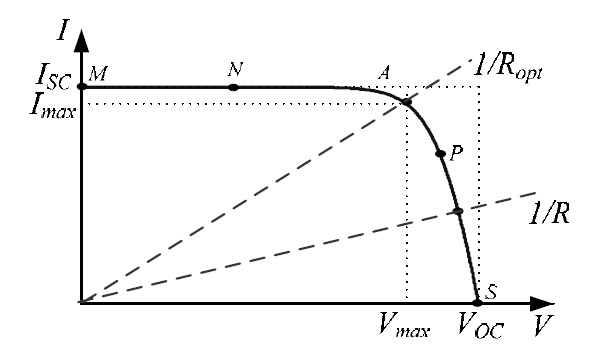
\includegraphics[scale=0.6]{./IV.jpg}
    \rule{35em}{0.5pt}
  \caption[Curva característica de corriente(A)-tensión(V) para un un panel fotovoltaico ]{Curva característica de corriente(A)-tensión(V) para un un panel fotovoltaico, (Tomado de $\left[2\right]$)}
  \label{fig:Curva_PV}
\end{figure}

La curva característica de un PV  se puede obtener manteniendo fijos los parámetros de irradiancia(S) y temperatura(T), en condiciones controladas. Si se tiene una carga en las terminales de salida, la potencia entregada solo dependerá del valor de la carga, de manera que si la carga es pequeña (puntos M-N de la figura \ref{fig:Curva_PV}) el panel se comportará como una fuente de corriente, pero si la carga es grande (puntos PS de la figura \ref{fig:Curva_PV}) se comportará como una fuente de tensión [2]. 

Para realizar la caracterización de una celda se deben realizar las siguientes pruebas: 

\begin{compactitem}

\item \nt{Corriente de corto circuito $\ I_{sc}$ }: Se define como el valor máximo de la corriente generada por el panel, en condiciones de cortocircuito $\ V=0$.


\item \nt{Tensión de circuito abierto $\ V_{oc}$}: Se define como el valor de tensión en la junta \nt{p-n}, cuando se tiene una corriente generada $\ I=0$.

\item  \nt{Punto de máxima potencia}: El punto A de la figura \ref{fig:Curva_PV} representa la potencia máxima de la carga resistiva,  $\ P_{max} = V_{max}I_{max}$.


\end{compactitem}



\subsection{Modelos del panel fotovoltaico}

Un panel fotovoltaico se puede modelar de manera simple (ideal), utilizando una fuente de corriente en paralelo con un diodo, la corriente de salida será proporcional a la radiación solar sobre la celda (foto-corriente). 

\begin{figure}[H]
  \centering
    \includegraphics[scale=0.07]{./M1PV.png}
    \rule{35em}{0.5pt}
  \caption[Modelo simple ideal para un panel fotovoltaico, compuesto por un diodo y una fuente de corriente]{ Modelo simple ideal para un panel fotovoltaico, compuesto por un diodo y una fuente de corriente}
  \label{fig:Modelo1_PV}
\end{figure}

La figura \ref{fig:Modelo1_PV} muestra el modelo básico, sin embargo este se puede realizar de una manera mas compleja, incluyendo variables para las características del panel: 

\begin{compactitem}

\item Dependencia de la temperatura, corriente de saturación del diodo (\nt{Is}) y foto corriente (\nt{Ig})


\item Pérdidas debidas al flujo de corriente (\nt{Rs}) y pérdidas con referencia a tierra (\nt{Rp}).

\item  número de celdas en análisis \nt{n}.

\end{compactitem}

\begin{figure}[H]
  \centering
    \includegraphics[scale=0.07]{./M2PV.png}
    \rule{35em}{0.5pt}
  \caption[Modelo para un panel fotovoltaico, compuesto por un diodo, una fuente de corriente, perdidas resistivas por cada celda]{ Modelo para un panel fotovoltaico, compuesto por un diodo, una fuente de corriente, perdidas resistivas por cada celda}
  \label{fig:Modelo2_PV}
\end{figure}

A partir del modelo con pérdidas se puede deducir la ecuación que describe las corrientes $ i_{pv}$ e $ I_{g}$ , como sigue a continuación [4]:

\begin{equation} \label{eq:ej1}
  i_{pv}
  = I_{s} - i_{d} + i_{p}
\end{equation}

\begin{equation} \label{eq:ej2}
  I_{g}
  =
  2i_{pv} + \frac{V_{pv}+i_{pv}R_{s}}{R_p} -  I_{s} + I_{s}e^{ \frac{V_{pv}+i_{pv}V_{pv}}{n v_t}} 
\end{equation}

\textsl{Despejando $\ i_{pv}$}

\begin{equation} \label{eq:ej3}
  i_{pv} 
  =
  \frac{1}{2} \left[I_{s} + I_{g} - \frac{V_{pv}+i_{pv}R_{s}}{R_p} - I_{s}e^{ \frac{V_{pv}+i_{pv}V_{pv}}{n v_t}} \right]
\end{equation}
  
  
En general, la corriente que fluye por las terminales de un generador fotovoltaico está determinada por tres funciones de corriente:
\begin{compactitem}
\item \nt{Ig}: Corriente generada debido al efecto fotoeléctrico.
\item \nt{id}: Corriente de pérdida debido a la juntura p-n.
\item \nt{ip}: Corriente de pérdida de naturaleza resistiva.
\end{compactitem}


 Para obtener un modelo del comportamiento estático del generador fotovoltaico se supone lo siguiente:

\begin{compactitem} 
\item \nt{Ig}: depende de la Irradiancia (S), pero no depende de la tensión en las terminales del generador fotovoltaico (\nt{Vpv})
\item \nt{ip} e \nt{id}: dependen de la tensión \nt{Vpv}
\item \nt{ip}: Depende de la temperatura (T)
\end{compactitem}

De esta forma, la expresión que define $\ i_{pv}$:

\begin{equation} \label{eq:ej4}
  i_{pv} \left(V_{pv},T,S \right) 
  =
  i_g \left(V_{pv}\right)-i_d \left(V_{pv},T\right)
\end{equation}

Según se definan las funciones $\ i_{pv}$ e $\ i_{d}$, se obtendrán modelos con complejidad y precisiones distintas, a partir de los siguientes casos: 


\begin{table}[H]
\centering
\caption{Modelos para un PV: ideal, con pérdidas en serie $\ R_s$  y con pérdidas en paralelo $\ R_p$ }
\label{Table:Modelos}
\begin{tabular}{|l|c|c|c|}
\hline
Modelos                                                             & $\ i_g$     & $\ i_p$ & $\ i_d$       \\ \hline
\begin{tabular}[c]{@{}c@{}} 1
\end{tabular}  & $\ KS $ & -   & $\ I_s\left(T\right)\left[e^\frac{V_{pv}}{v_t}-1\right] $          \\ \hline
\begin{tabular}[c]{@{}c@{}} 2
\end{tabular} & $\ KS $ & $\ G_pV_{pv} $   & $\ I_s\left(T\right)\left[e^\frac{V_{pv}}{v_t}-1\right] $          \\ \hline

\begin{tabular}[c]{@{}c@{}} 3 
\end{tabular} & $\ KS $ & -   & $\ I_s\left(T\right)\left[e^\frac{V_{pv} + i_{pv}R_{s} }{v_t}-1\right] $          \\ \hline
\begin{tabular}[c]{@{}l@{}} 4
\end{tabular} & $\ KS $ & $\ G_pV_{pv} + G_pi_{pv}R_s $   & $\ I_s\left(T\right)\left[e^\frac{V_{pv} + i_{pv}R_{s}}{v_t}-1\right] $     \\ \hline

\end{tabular}
\end{table}

De manera general se tiene: 

\begin{equation} \label{eq:ej5}
  i_{pv} \left(V_{pv}\right) 
  =
  G_{p}V_{pv} + G_{p}i_{pv}R_s
\end{equation}


\begin{equation} \label{eq:ej6}
  i_{d} \left(V_{pv}\right) 
  =
  I_s \left(T \right) e^\frac{V_{pv}}{v_t} e^\frac{ i_{pv}R_{s}}{v_t} -I_s \left(T \right)
\end{equation}

El modelo general del comportamiento estático de un generador PV, también se puede representar de la siguiente manera: 

\begin{equation} \label{eq:ej7}
  i_{pv}  
  =
  KS - G_{p}V_{pv} + I_s \left(T \right) - G_{p}i_{pv}R_s - I_s \left(T \right) e^\frac{V_{pv}}{v_t} e^\frac{ i_{pv}R_{s}}{v_t} 
\end{equation}

\begin{equation} \label{eq:ej8}
  I_s \left(T \right) e^\frac{V_{pv}}{v_t} e^\frac{ i_{pv}R_{s}}{v_t}   
  =
  KS - G_{p}V_{pv} + I_s \left(T \right) - G_{p}i_{pv}R_s - i_{pv} 
\end{equation}

La ecuación \ref{eq:ej8} es no lineal, aplicando una linealización, se tiene [3]: 

\begin{equation} \label{eq:ej9}
  y = ln \left(KS - G_{p}V_{pv} + I_s \left(T \right) - G_{p}i_{pv}R_s - i_{pv} \right) 
\end{equation}

si $ I_g = KS >> I_s $

\begin{equation} \label{eq:ej10}
  y = ln \left(KS - G_{p}V_{pv} - G_{p}i_{pv}R_s - i_{pv} \right) 
\end{equation}

\begin{equation} \label{eq:ej11}
  z = V_{pv} + i_{pv}R_s  
\end{equation}

Posteriormente al proceso de cálculo de parámetros se tiene: 

\begin{equation} \label{eq:ej12}
  \theta_1  = ln\left( I_s \left(T \right) \right)
\end{equation}

\begin{equation} \label{eq:ej13}
  \theta_2  = \alpha 
\end{equation}

\section{Algoritmo de CORDIC}

El algoritmo \nt{Coordinate Rotational Digital Computer} (CORDIC) es un método numérico, en donde se realiza cierto número de iteraciones para encontrar el valor deseado, según sea la función que se desea calcular. Este algoritmo es utilizado para implementar funciones trigonométricas, logarítmicas y  exponenciales. La facilidad de implementación, hace que sea uno de los algoritmos más utilizados en el ámbito de la electrónica digital. CORDIC implementado digitalmente utiliza desplazamientos, sumas, restas y tablas look-up con valores previamente precargados en una memoria ROM, que dependerán de la operación en cálculo. Para este algoritmo existe: el método circular, lineal e hiperbólico.   

Las ecuaciones generales para el algoritmo de CORDIC se definen como: 

\begin{equation} \label{eq:ej14}
  X_{i+1} = X_{i}- md_{i} 2^{-i} Y_{i}  
\end{equation}

\begin{equation} \label{eq:ej15}
  Y_{i+1} = Y_{i}- d_{i} 2^{-i} X_{i}  
\end{equation}

\begin{equation} \label{eq:ej16}
  Z_{i+1} = Z_{i}- d_{i} e\left(i\right)
\end{equation}

Donde $\ e\left(i\right) $ se muestra en la tabla \ref{Table:ei} según corresponde cada caso:

\begin{table}[H]
\centering
\caption{Sistema de coordenadas unificado (CORDIC): circular, linear e hiperbólico. Tomado de [5]}
\label{Table:ei}
\begin{tabular}{|l|c|c|c|}
\hline
m & Sistema de coordenadas                                                             & Valor de $\ e\left(i\right) $     \\ \hline
\begin{tabular}[c]{@{}c@{}} 1
\end{tabular}  & Circular & $\ tan^{-1}\left(2^{-i}\right)$         \\ \hline
\begin{tabular}[c]{@{}c@{}} 0
\end{tabular} & Lineal & $\ 2^{-1} $          \\ \hline

\begin{tabular}[c]{@{}c@{}} -1 
\end{tabular} & Hiperbólico & $\ tanh^{-1}\left(2^{-i}\right)$                \\ \hline


\end{tabular}
\end{table}



\subsection{Sistema de coordenadas hiperbólico}

Para el cálculo de algunas funciones con el algoritmo aumenta la complejidad, de manera que se deben utilizar las siguientes identidades [6]:

\begin{equation} \label{eq:ej17}
  \tan z = \frac{\sin z}{\cos z}
\end{equation}

\begin{equation} \label{eq:ej18}
  \tanh z = \frac{\sinh z}{\cosh z}
\end{equation}

\begin{equation} \label{eq:ej19}
  \exp z = \sinh z + \cosh z
\end{equation}

\begin{equation} \label{eq:ej20}
  \ln \omega = 2 \tanh^{-1} \left( \frac{y}{x} \right)
\end{equation}

Donde: 

\begin{equation} \label{eq:ej21}
  x = \omega + 1
\end{equation}

\begin{equation} \label{eq:ej22}
  y = \omega - 1
\end{equation}

\subsection{Logaritmo natural utilizando el algoritmo hiperbólico de CORDIC}
Para la función $\ Ln \left(\omega\right) $, utilizado el algoritmo de CORDIC en modo hiperbólico [12], se debe calcular primeramente la función $\ \tanh^{-1} \left( \frac{y}{x} \right)$ a partir de las siguientes ecuaciones:

 
\begin{equation} \label{eq:ej23}
  X_{i+1} = X_{i} + d_{i} 2^{-i} Y_{i}  
\end{equation}

\begin{equation} \label{eq:ej24}
  Y_{i+1} = Y_{i} + d_{i} 2^{-i} X_{i}  
\end{equation}

\begin{equation} \label{eq:ej25}
  Z_{i+1} = Z_{i} - d_{i} tanh^{-1}\left(2^{-i}\right)
\end{equation}

Donde $\ i $ es el indice de cada iteración. Las iteraciones 4, 13, 40,… k, 3k+1 se deberán repetir para garantizar la convergencia. $\ d_i $ es el signo de $\ Y_i $ invertido, es decir el cuando el signo de $\ Y_i $ es negativo, $\ d_i $ será positivo y viceversa.

Utilizando la ecuación \ref{eq:ej20}, se definen los valores iniciales   $\ X_0 = \omega + 1$ , $\ Y_0 = \omega - 1$ y $\ Z_0 = 0 $, cuando $\ i = 0 $.

Cabe destacar que el rango de convergencia para este algoritmo [7] esta definido como: 

\begin{equation} \label{eq:ej26}
   0,106843 \leq \omega \leq 9,35947
\end{equation}

Donde $\ \omega $ es el valor del argumento del logaritmo natural.

El resultado final de $\ Z_i $, contiene el valor de $\ \tanh^{-1} \left( \frac{y}{x} \right)$, sin embargo se debe multiplicar por un factor de 2 para completar el cálculo del logaritmo natural, según la identidad de la ecuación \ref{eq:ej20} 

\subsection{Exponencial utilizando el algoritmo hiperbólico de CORDIC }


Para una función  $\ e^{\left(\omega\right)} $, con el algoritmo de CORDIC, se debe utilizar las ecuaciones \ref{eq:ej23}, \ref{eq:ej24} y \ref{eq:ej25} de manera iterativa, donde el valor final de $\ X $ y $\ Y$, son el resultado de $\\cosh\left(\omega\right)$ y $\ \sinh\left(\omega\right)$ respectivamente. Se debe tomar en cuenta la repetición de las iteraciones $\ \left(i\right) $ 4, 13, 40,… k, 3k+1 para garantizar la convergencia dando una mejor precisión en el cálculo.

Los valores iniciales se definen como \nt{constantes} $\ X_0 = 1,20753406 $ , $\ Y_0 = 0$ y $\ Z_0 = \omega $, donde $\ \omega$,  es el valor del argumento que se desea calcular, y $\ d_i $ es el signo de $\ Z_i $.

Cabe destacar que el rango de convergencia para este algoritmo se puede definir como: 

\begin{equation} \label{eq:ej26}
   0 \leq \omega \leq 1
\end{equation}

El valor final del cálculo, se obtiene por medio de una suma de dos funciones, dadas en la identidad de la ecuación \ref{eq:ej19}. 

\section{Coma flotante}

La codificación para el formato coma flotante se realiza mediante el estándar \nt{IEEE 754}, este requiere de tres campos en la palabra [10]: 

\begin{compactitem}
\item Signo 
\item Exponente
\item Mantisa 
\end{compactitem}

\begin{figure}[H]
  \centering
    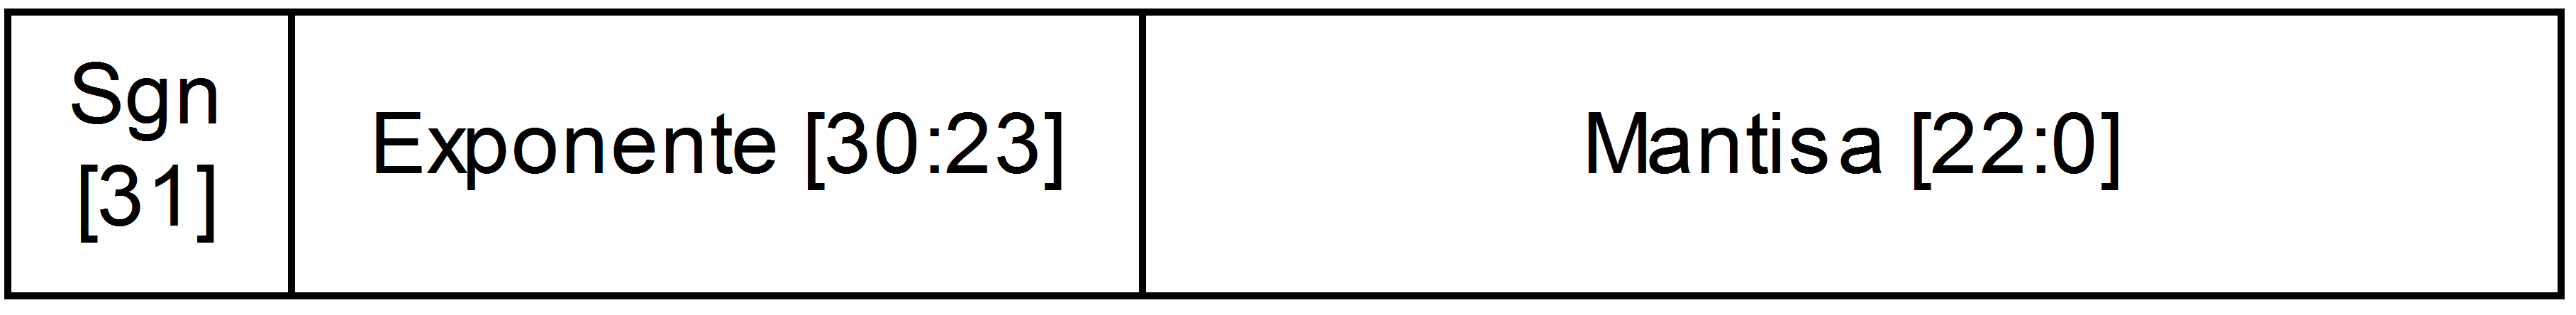
\includegraphics[scale=0.08]{./FLOAT.png}
    \rule{35em}{0.5pt}
  \caption[Formato IEEE 754 coma flotante para 32 bits]{Formato IEEE 754 coma flotante para 32 bits}
  \label{fig:FLOAT}
\end{figure}

Para el formato \nt{IEEE 754} de la figura \ref{fig:FLOAT} en 32-bits [8] se asigna: 

\begin{compactitem}
\item 1 Bit para signo 
\item 8 Bits para exponente
\item 23 Bits para mantisa 
\end{compactitem}

Donde el bit de signo representa un numero positivo si este es 0, de manera contraria representa un número negativo. 

El exponente (8-bits) puede representar un rango desde 0 hasta 255, sin embargo se tiene:

\begin{compactitem}
\item $\ \left[0-127\right]$ exponentes negativos  
\item $\ \left[128-255\right]$ exponentes positivos
\end{compactitem}

De esta manera para convertir un exponente positivo, en el valor correspondiente del formato coma flotante se debe realizar la siguiente suma: $\ exp_{float}=127+exp_numero $. Por otro lado si se desea pasar de un valor decimal a coma flotante se deben realizar los siguientes pasos: 

\begin{compactitem}
\item Representar el signo con su debido bit
\item Conversión decimal a binario coma fija   
\item Conversión binario a notación científica
\item Agrupar en signo, exponente y mantisa 
\end{compactitem}


\section{Coma fija}
 
La representación de un número en coma fija cuenta con tres partes fundamentales:
\begin{compactitem}
\item Signo
\item Parte entera   
\item Parte fraccionaria 
\end{compactitem}

\begin{figure}[H]
  \centering
    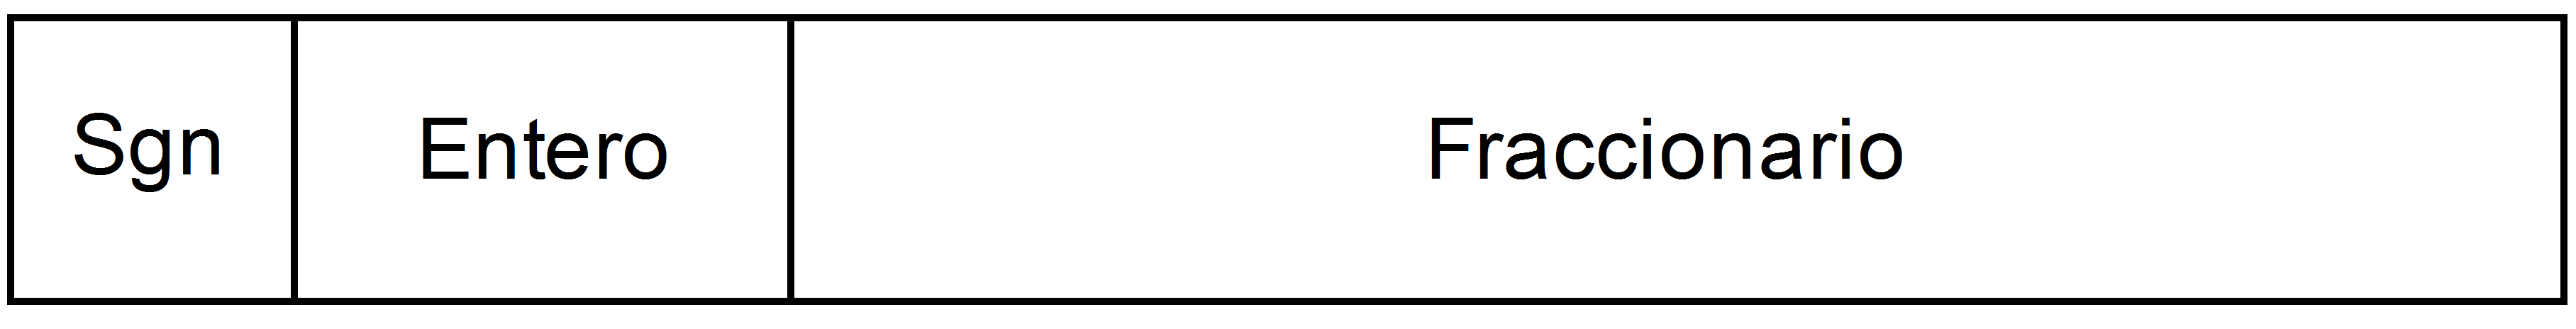
\includegraphics[scale=0.08]{./FIXED.png}
    \rule{35em}{0.5pt}
  \caption[Formato para un número en coma fija]{Formato para un número en coma fija}
  \label{fig:FIXED}
\end{figure}

En la aritmética simple se utilizan los signos +/-, para saber si un número es positivo o negativo, para representar el signo en coma fija se utiliza el bit mas significativo. Si el número es positivo, el bit de signo será un 0 y si el número es negativo, será un 1 [13]. Si se requiere de una representación de un numero negativo en coma fija, se debe utilizar el complemento a 2 [14]. La coma se asigna de manera arbitraria según se requiera.  
 
  